\subsection{Poisson problem}
In this section, the Poisson problem is revisited and implemented to run on a GPU. The Poisson problem is memory bound, and thus the limiting factor of the computation is the memory bandwidth to the cores. In all three subsequent subsections, the memory is initialized on the CPU and then transferred to the GPU for computations, and transferred back in the end.

\subsubsection{Single thread on GPU}
Again, we begin by implementing a kernel that runs exactly like the sequential CPU version, but on the GPU. This ensures that the cuda framework is correct, and that the kernel produces the right result. The framework is shown below, with the source code of \texttt{jacobi\_seq\_kernel} is identical to the sequential version in project 2. 

\begin{lstlisting}
	cudaMalloc(&d_u, memsize);
	cudaMalloc(&d_uo, memsize);
	cudaMalloc(&d_f, memsize);	
	cudaMemcpy(d_u, u, memsize, cudaMemcpyHostToDevice);
	cudaMemcpy(d_uo, uo, memsize, cudaMemcpyHostToDevice);
	cudaMemcpy(d_f, f, memsize, cudaMemcpyHostToDevice);

	int k = 0;
	while(k < kmax){
		jacobi_seq_kernel<<<1, 1>>>(d_u, d_uo, d_f, N, delta2);
		double * temp = d_uo;
    		d_uo = d_u;
    		d_u = temp;
		k++;
	}

	cudaMemcpy(uo, d_uo, memsize, cudaMemcpyDeviceToHost);
	cudaFree(d_u);
	cudaFree(d_uo);
	cudaFree(d_f);
\end{lstlisting}
In this project we do not consider the convergence, and thus, the program iterates until a user-specified maximum is reached. The timing of the function is measured for different matrix sizes ranging from $16\times 16$ to $256\times 256$ and compared to our best implementation from week2 (\texttt{omp3}). On figure \ref{fig:poisson_seq} point updates per second for \texttt{omp3} running on a single core and the sequential GPU implementation can be seen.

\begin{figure}
\centering
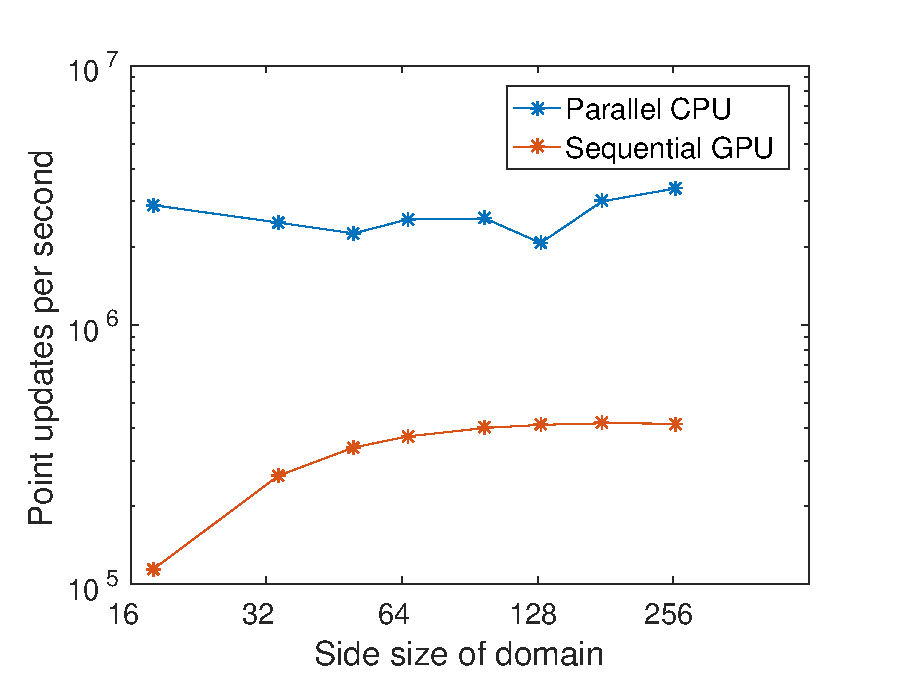
\includegraphics[width = 0.8\textwidth]{fig/gpuseq.eps}
\caption{1-core OMP and sequential GPU implementations}
\label{fig:poisson_seq}
\end{figure}


\subsubsection{Naive version with 1 thread per element}
One thread to do all the work is obviously not good, so we implement a naive version of one thread per element of the matrices. Per iteration, each thread loads 5 values (4 neighbours from $u_o$ and 1 from $f$) and performs 6 Flops, and the problem is thus memory bound. One implementation note is that for the Poisson problem only inner grid points are updated. This means that the total number of threads needed (when entire matrix is $N x N$) is $(N-2)^2$ and the grid size should be specified accordingly. Since the block and thread numbers start from 0 it is therefore necessary to add 1 to the row and column values in jacobi kernel function. Visually this is just shifting an $N-2 x N-2$ window on an $N x N$ matrix so it covers just the inner points.  

\begin{lstlisting}
	double *d_u, *d_uo, *d_f;
	int memsize = N*N*sizeof(double);
	cudaMalloc(&d_u, memsize);
	cudaMalloc(&d_uo, memsize);
	cudaMalloc(&d_f, memsize);	
	cudaMemcpy(d_u, u, memsize, cudaMemcpyHostToDevice);
	cudaMemcpy(d_uo, uo, memsize, cudaMemcpyHostToDevice);
	cudaMemcpy(d_f, f, memsize, cudaMemcpyHostToDevice);
	int k = 0;
	double checksum = 1000.0;	
	cudaSetDevice(6);
	int K = 16;
	int gridx = ceil((N-2)*1.0/(K));
	int gridy = ceil((N-2)*1.0/(K));
	double start = omp_get_wtime(); 
	while(k < kmax){
		jacobi_single_kernel<<<dim3(gridx,gridy),dim3(K,K)>>>(d_u, d_uo, d_f, N, delta2);
		double * temp = d_uo;
    		d_uo = d_u;
    		d_u = temp;
		k++;
	}
\end{lstlisting}

\begin{lstlisting}
__global__ 
void jacobi_single_kernel(double * d_u, double * d_uo, double * d_f, int N, double delta2){
	int j = blockIdx.x * blockDim.x + threadIdx.x + 1;
	int i = blockIdx.y * blockDim.y + threadIdx.y + 1;
	if (j < N-1 && i < N-1){
		d_u[i*N + j] = 0.25*(d_uo[(i-1)*N + j] + d_uo[(i+1)*N + j] + d_uo[i*N + j+1] + d_uo[i*N + j-1] + delta2*d_f[i*N + j]);
	}
}
\end{lstlisting}

Figure \ref{fig:poisson_seq} presents the point updates per second for \texttt{omp3} running on 14 threads and the naive GPU approach. It is apparent that the naive GPU approach already easily outperforms our best implementation from week2.  


\begin{figure}
\centering
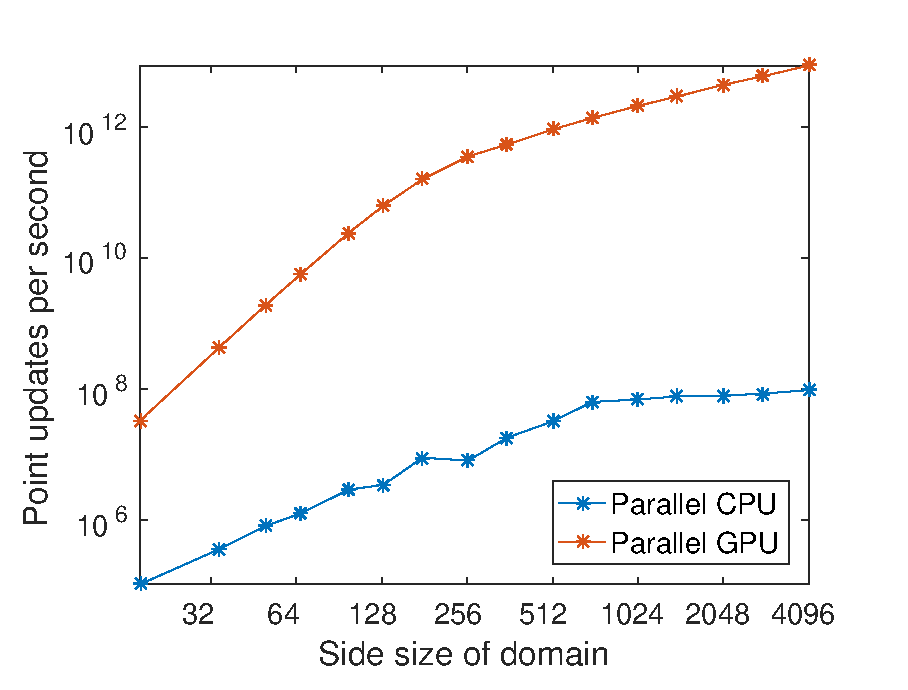
\includegraphics[width = 0.8\textwidth]{fig/gpupar.eps}
\caption{Poisson problem performance for our best CPU and naive GPU implementations}
\label{fig:poisson_sin}
\end{figure}

\textbf{SOMETHING ABOUT PROFILING OF SIN HERE. THE PROFILING NODE WAS/IS OVERUSED}
For improvements, an obvious choice would be to implement the shared memory used in \texttt{gpu5} is the matmult exercise, but since each point is only used by its neighbours, most points will be used inside a single block, enabling the automatic cache control to do quite well. For the blocking to be really effective, the blocks should be iterated multiple times between being synchronized. If the blocks do e.g. 10 iterations isolated from the rest of the blocks, the flops/element would increase by a factor of 10 also. The number of iterations should be chosen to match the optimum match between flops and memory for the GPU used. This procedure would require additional calculations to get the edges of the blocks correct, but it would still be beneficial. Another optimization would be to have the loop and the pointer swap on the GPU. That way, each block could have a copy of its relevant region of $f$ in the cache all the time, which would reduce the memory transfer from the global memory by a third, leaving more bandwidth for transferring $u$ and $u_o$.


\subsection{Multi-GPU}
Adjusting the naive version to run on two GPUs entails splitting the matrices in two and updating the values in parallel. Special consideration needs to be placed on the points near the boundary of the splits since updating these points requires values from the other split. We made the simplifying assumption that $N$ is even, in our case the two splits thus correspond to the first and last $N/2$ rows of the matrices. We allocate memory and copy the upper and lower parts of the matrices with an additional row that is not updated but used solely for calulating the boundary rows' values.
Since these additional rows are not updated, it is necessary to 'refresh' the rows on each iteration by copying the correct row from the other split. Since updating the lower and upper splits of the matrix are conceptually the same, i.e. both update only the inner points, a single kernel implementation can be used.


\begin{lstlisting}
double *d0_u, *d0_uo, *d0_f, *d1_u, *d1_uo, *d1_f;
	int memsize = N*N*sizeof(double);
	int Nsize = N*sizeof(double);

	cudaSetDevice(6);
	cudaDeviceEnablePeerAccess(7,0);
	cudaMalloc((void**)&d0_u, memsize/2 + Nsize);
	cudaMalloc((void**)&d0_uo, memsize/2 + Nsize);
	cudaMalloc((void**)&d0_f, memsize/2 + Nsize);
	cudaMemcpy(d0_u, u, memsize/2 + Nsize, cudaMemcpyHostToDevice);
	cudaMemcpy(d0_uo, uo, memsize/2 + Nsize, cudaMemcpyHostToDevice);
	cudaMemcpy(d0_f, f, memsize/2 + Nsize, cudaMemcpyHostToDevice);

	cudaSetDevice(7); 
	cudaDeviceEnablePeerAccess(6,0);
	cudaMalloc((void**)&d1_u, memsize/2 + Nsize);
	cudaMalloc((void**)&d1_uo, memsize/2 + Nsize);
	cudaMalloc((void**)&d1_f, memsize/2 + Nsize);
	cudaMemcpy(d1_u, &u[memsize/2/sizeof(double) -N], memsize/2 + Nsize, cudaMemcpyHostToDevice);
	cudaMemcpy(d1_uo, &uo[memsize/2/sizeof(double) -N], memsize/2 + Nsize, cudaMemcpyHostToDevice);
	cudaMemcpy(d1_f, &f[memsize/2/sizeof(double) -N], memsize/2 + Nsize, cudaMemcpyHostToDevice);
	int k = 0;
	double checksum = 1000.0;	
	int K = 16;
	int gridx = ceil((N-2)*1.0/(K));
 	int gridy = ceil((N-2)*1.0/(K));
	gridy = ceil(gridy*1.0 / 2);
	double start = omp_get_wtime(); 
	while(k < kmax){
		cudaSetDevice(6);
		jacobi_multi_kernel<<<dim3(gridx,gridy),dim3(K,K)>>>(d0_u, d0_uo, d0_f, N, delta2);
		cudaSetDevice(7);
		jacobi_multi_kernel<<<dim3(gridx,gridy),dim3(K,K)>>>(d1_u, d1_uo, d1_f, N, delta2);
		cudaDeviceSynchronize();
		double * temp = d0_uo;
    		d0_uo = d0_u;
    		d0_u = temp;
		double * temp2 = d1_uo;
		d1_uo = d1_u;
    		d1_u = temp2;
		cudaMemcpy(d1_uo, d0_uo+(N-2)/2*N, Nsize, cudaMemcpyDeviceToDevice);
		cudaMemcpy(d0_uo+(N-2)/2*N+N , d1_uo+N, Nsize, cudaMemcpyDeviceToDevice);
		k++;
	}
\end{lstlisting}


\begin{lstlisting}
__global__ 
void jacobi_multi_kernel(double * d_u, double * d_uo, double * d_f, int N, double delta2){
	int j = blockIdx.x * blockDim.x + threadIdx.x + 1;
	//int i = blockIdx.y * blockDim.y + threadIdx.y + 1;
	int i = blockIdx.y * blockDim.y + threadIdx.y + 1;
	if (j < N-1 && i < N/2 && j > 0 && i > 0){
		d_u[i*N + j] =  0.25*(d_uo[(i-1)*N + j] + d_uo[(i+1)*N + j] + d_uo[i*N + j+1] + d_uo[i*N + j-1] + delta2*d_f[i*N + j]);
	}	
}
\end{lstlisting}

On figure \ref{fig:poisson_mul} point updates per second for \texttt{omp3} and both single GPU and multi GPU implementations can be seen. Obviously the GPU aproaches greatly outperform the CPU approach. However, with our implementations, utilizing 2 GPUs brings no performance benefit. That is surprising as we were expecting a speedup factor close to 2 and thus we assume the problem is in our code. We verified using nvidia visual profiler that both GPUs were utilised in parallel and thus ruled out erroneous synchronization causing sequential execution. We also verified that the performance impact of the memcopy calls within the loop are insignificant compared to the entire computation. Additionally,  we saw that most of the time was spent in the jacobi kernel functions and that the number of kernel function calls was correct. 


\begin{figure}
\centering
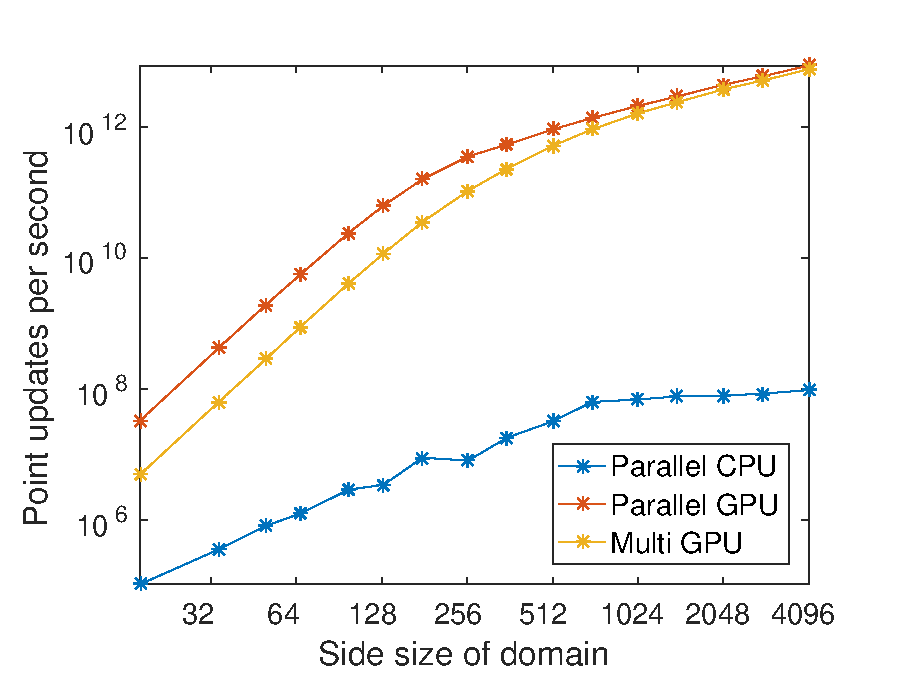
\includegraphics[width = 0.8\textwidth]{fig/multigpu.eps}
\caption{Poisson problem performance for our CPU and GPU implementations}
\label{fig:poisson_mul}
\end{figure}
